\chapter{Soluția propusă}
\section{Informații preliminare}
\subsection{Informații tehnice}
Pentru dezvoltarea, structurarea și versionarea codului sursă al lucrării, am folosit platforma gratuită Github\footnote{\url{https://github.com}}.
Repository-ul proiectului poate fi accesat la această adresă: \url{https://github.com/sergiuiacob1/iClicker/}.

Rezultatele prezentate aici au fost bazate pe imagini capturate prin intermediul unei camere webcam capabile de o rezoluție maximă HD (1280x720 pixeli).
Experimentele realizate au fost făcute în general în medii bine luminate, întrucât o dată cu scăderea intensității luminii suferă și utilitatea aplicației prezentate aici.

\subsection{Python \& Conda}
Unul dintre cele mai populare limbaje de programare când vine vorba de Învățare Profundă este Python.
Astfel, am ales să dezvolt aplicația folosind acest limbaj, deoarece suportul din partea comunității este unul foarte bun și resursele găsite online pentru a rezolva probleme comune sunt vaste.

Am facut uz de asemenea de tehnologia Conda care ajută în gestionarea mediilor de dezvoltare.
Cu ajutorul acestora am putut crea un mediu de dezvoltare separat, care se poate instala cu ușurință pe orice calculator fără a crea conflicte cu alte pachete deja existente pe mașina unui utilizator.
Această combinație a ajutat la îndeplinirea necesității aplicației de a rula pe mai multe sisteme de operare, întrucât Python deja satisface această nevoie.
Versiunile folosite au fost \lstinline{Python 3.7} și Conda \lstinline{4.8.0}.

\subsection{OpenCV}
Una dintre bibliotecile Python care au adus funcționalități cruciale acestui proiect este OpenCV.
Aceasta conține diferite funcționalități legate de Viziunea Computerizată, precum captura de imagini prin intermediul webcam-ului.
Am folosit-o de asemenea pentru a realiza redimensionări de imagini, pentru a le converti în gri sau în imagini alb-negru prin aplicarea unui \emph{binary threshold}.
Versiunea folosită a fost \lstinline{4.1.2}.

\subsection{PyQt5}
Aplicația dezvoltată are și o interfață grafică ce a fost implementată folosind biblioteca PyQt5.
Unul dintre avantajele acestei biblioteci este acela că oferă un nivel înalt de abstractizare și componentele (butoanele, ferestrele etc.) grafice au un aspect diferit în funcție de sistemul de operare pe care rulează aplicația, fără a fi nevoie ca acest lucru să fie implementat de dezvoltator.
Versiunea folosită a fost \lstinline{5.14}.

\subsection{Keras \& PyTorch}
Keras și PyTorch au fost folosite pentru a facilita antrenarea rețelelor neuronale (de tip \emph{MLP} sau \emph{CNN}).
Acestea au mărit cu mult realizarea arhitecturilor pentru învățarea automată, Keras având un nivel de abstractizare decât PyTorch.
Am folosit cele două tehnologii pentru a căpăta experiență în utilizarea amândurora, întrucât nu există o ``cea mai bună unealtă'', ci mai degrabă contextul nevoii dictează uneltele, tehnologiile ce ar trebui folosite.
Versiunile folosite au fost \lstinline{Keras 2.2.4} și PyTorch \lstinline{1.4}.

\subsection{dlib}
Cea mai importantă bibliotecă de care am făcut uz în această lucrare este dlib.
Cu ajutorul acesteia, am putut realiza identificarea reperelor faciale într-o imagine care conținea fața unei persoane.
Reperele respective sunt furnizate de către sub forma unei liste de coordonate $(x, y)$ corespunzătoare pixelilor acelor caracteristici faciale.
Mai departe, pe baza acestora, am putut decupa fie fața, fie ochii persoanei în imagini mai mici pe care le-am folosit mai apoi ca date de antrenament.
Versiunea folosită a fost \lstinline{19.19.0}.

\section{Limite și constrângeri}
Aplicația are niște limite și lucrează de asemenea cu niște presupuneri, precum faptul că utilizatorul folosește un singur monitor și un singur webcam.
De asemenea, imaginile folosite sunt cu mine însumi, deci trebuie luat acest lucru pentru orice rezultat prezentat.

Aplicația este menită să se poată ``mula'' pe fizionomia utilizatorului, însă este posibil să aibă performanțe mai slabe pentru persoanele care poartă ochelari.
Motivul pentru care se întâmplă acest lucru este acela că aplicația lucrează cu ochii utilizatorului, iar dacă lumina se reflectă în lentilele ochelarilor, ochii ar putea fi indistinctibili.
Ca o ultimă mențiune, aplicația se concentrează majoritar pe poziția pupilelor relativ la ochi (glob ocular + anexe ale globului ocular), deci se va considera că poziția capului nu va suferi schimbări majore între datele de antrenament și datele de test.

\section{Structura aplicației}
Aplicația are 4 mari componente, corespunzătoare pașilor luați în rezolvarea unei probleme de învățarea automată: colectarea de date, procesarea acestora, antrenarea unei rețele convoluționale care realizează urmărirea ochilor și simularea funcționalităților mouse-ului.
Utilizatorul poate interacționa cu aceste componente prin intermediul interfaței grafice realizată în PyQt5.

Pentru a construi aplicația m-am ghidat după modelul de proiectare \emph{MVC} (\emph{Model–View–Controller}).
Fiecare componentă care poate fi folosită de utilizator are o interfață grafică atașată (\emph{View}) ce poate cere aplicației (prin intermediul unui \emph{Controller}) să realizeze anumite proceduri.
Partea de \emph{Model} al acestui tipar de dezvoltare constă în structurarea datelor colectate neprelucrate și a celor rezultate din partea de procesare a datelor.

\begin{figure}[H]
    \centering
    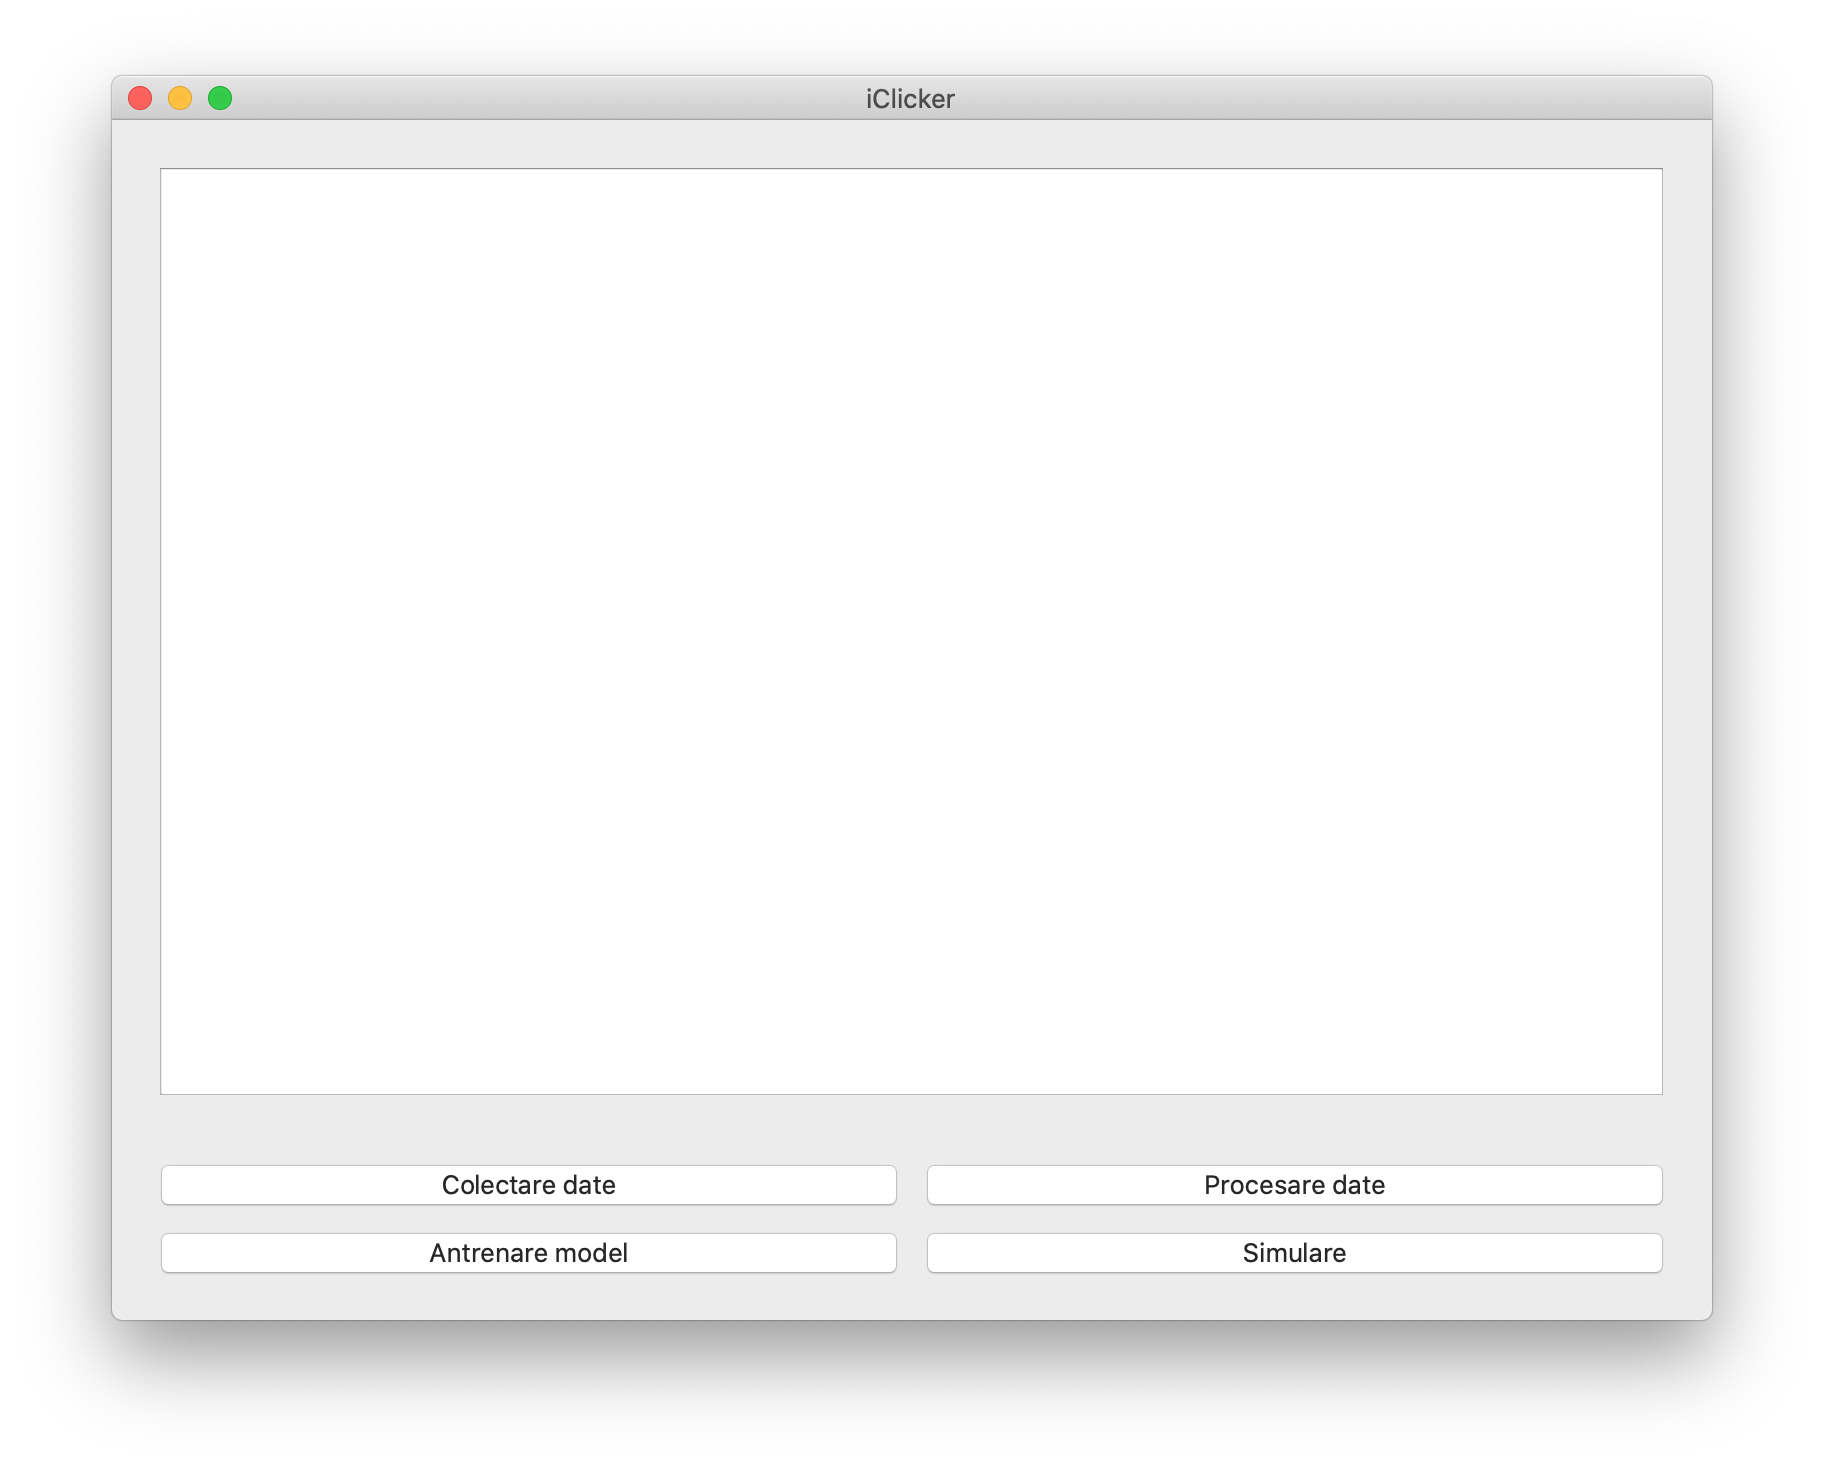
\includegraphics[width=\textwidth]{iClicker.png}
    \caption{Fereastra principală a aplicației}
\end{figure}

\begin{figure}[ht]
    \centering
    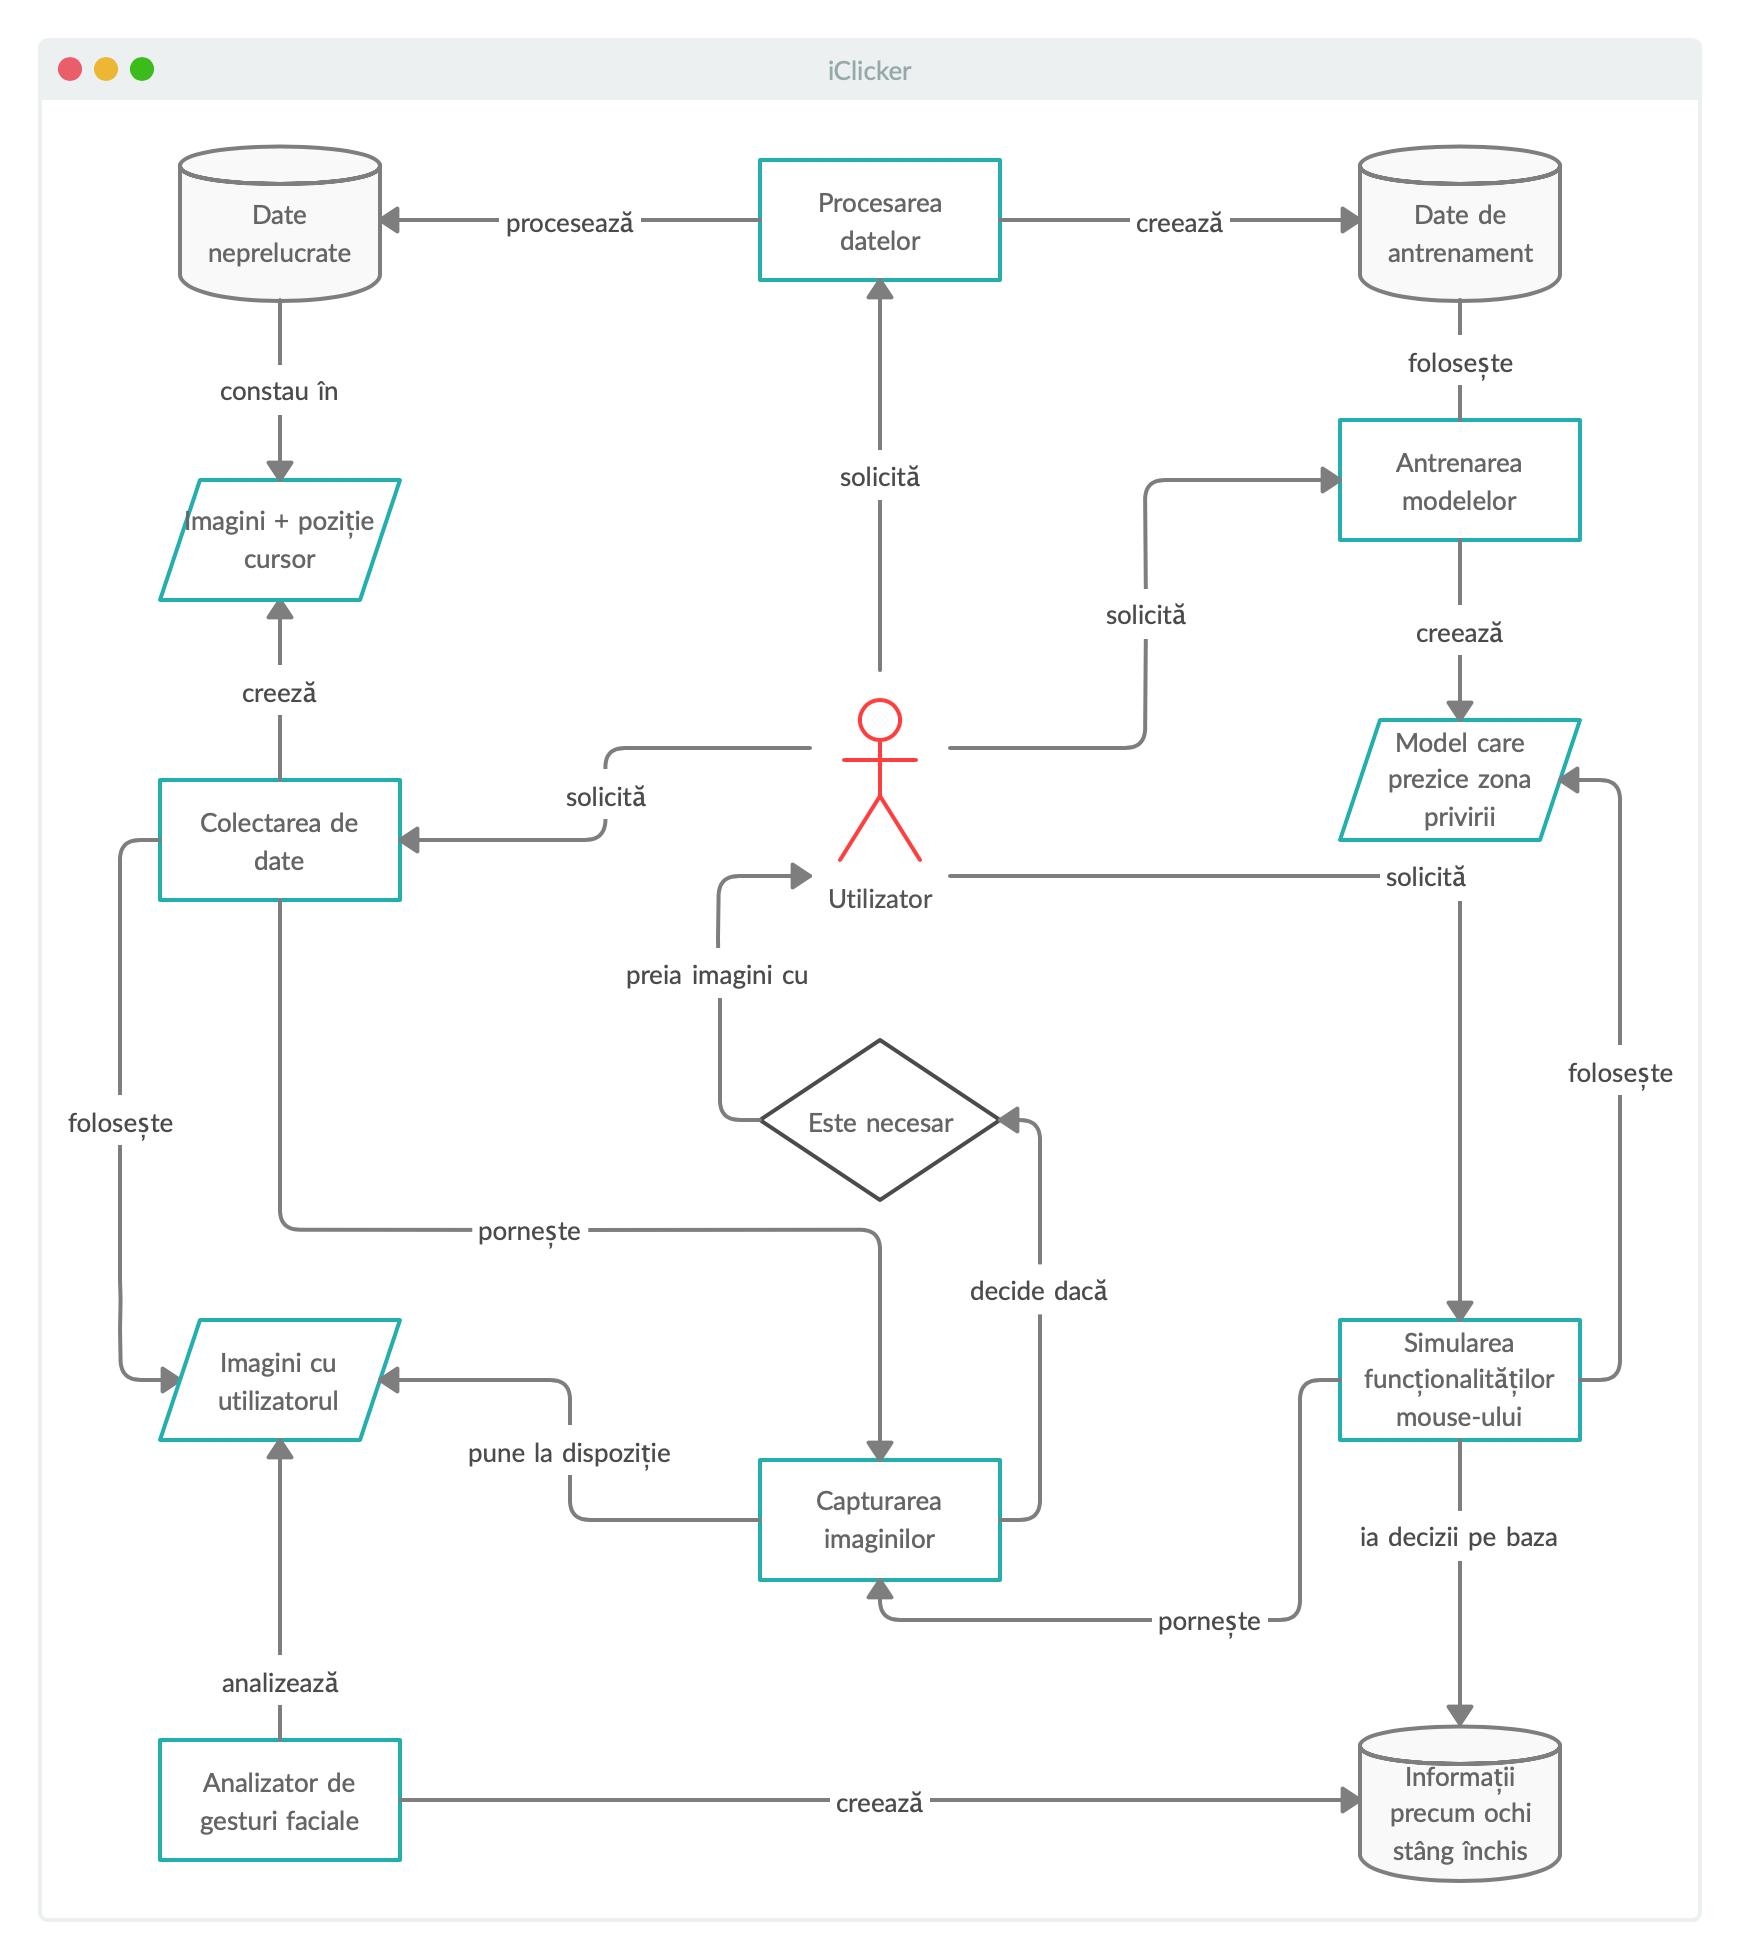
\includegraphics[width=\textwidth]{flowchart.png}
    \caption{Organigrama aplicației}
\end{figure}

\subsection{Colectarea de date}
Pentru a realiza această funcție, utilizatorul trebuie să apese pe butonul denumit sugestiv ``Colectare date''.

\subsection{Procesarea datelor}
\subsection{Antrenarea unui model}
\subsection{Predictie}